%Text Books : \cite{royden}
%Module 1: Lebesgue Measure
%Introduction, Lebesgue outer measure, The $\sigma$-algebra of Lebesgue measurable sets, Outer and inner approximation of Lebesgue measurable sets , Countable additivity, continuity and Borel-Cantelli Lemma, Non measureable sets, The Cantor set and Cantor Lebesgue function
%Chapter 2; Sections 2.1 to 2.7 (25 Hours)
%Module 2: Lebesgue Measurable Functions and Lebesgue Integration
%Sums, Products and Compositions, Sequential Pointwise Limits and Simple Approximation, The Riemann Integral, The Lebesgue Integral of a bounded measurable function over a set of finite measure, The Lebesgue Integral of a measurable non-negative function, The General Lebesgue Integral.
%Chapter 3; Sections 3.1 to 3.2, Chapter 4; Sections 4.1 to 4.4(25 Hours) 
%Module 3: General Measure Space and Measureable Functions \& Signed Measures
%Measures and Measurable Sets
%The Hanh and Jordan decompositions, The Caratheodory Measure induced by an outer measure, Measureable functions
%Chapter 17; Sections 17.1 to 17.3, Chapter 18; Section 18.1 upto corollory 7 (20 Hours)
%Module 4: Integration over General Measure Space and Product Measure
%Integration of non-negative meaurable functions, Integration of General Measurable functions, The Radon Nikodym Theorem
%The Theorems of Fubini and Tonelli
%Chapter 18; Sections 18.2 to 18.4, Chapter 20; Section 20.1 (20 Hours)

%Need to work on this
%Module 1 - \cite{royden} 2
%Module 2 - \cite{royden} 3, 4
%Module 3 - \cite{royden} 17, 18
%Module 4 - \cite{royden} 18, 20
%Missing - \cite{royden} 1, 5, 6, 7, 8, 9, 10, 11, 12, 13, 14, 15, 16, 19, 21?

\section{Lebesgue Measure}
\begin{description}
	\item[set function] A function which maps sets into (extended) real numbers.
	\item[$\sigma$-algebra] A family $\mathcal{A}$ of subsets of a nonempty set $X$ such that
	\begin{enumerate}
		\item $\mathcal{A}$ contains the empty set, 
		\item $\mathcal{A}$ contains complement of each of its members and
		\item $\mathcal{A}$ is closed under countable unions.
	\end{enumerate}
	
	From these 3 axioms, we can deduce the following,
	\begin{enumerate}
		\setcounter{enumi}{3}
		\item $\mathcal{A}$ is closed under countable intersections (by de Morgan's laws).
			$$\left( \bigcup_{k = 1}^\infty E_k^c \right)^c = \bigcap_{k=1}^\infty E_k \in \mathcal{A}$$
		\item $E,F \in \mathcal{A} \implies E-F \in \mathcal{A}$ since $E-F = E \cap F^c$
	\end{enumerate}
\end{description}

\begin{definition}[Length of an interval]
	Length is a real valued set function.
	Let $I$ be a bounded interval say $[a,b)$.
	Then its length $l(I)=b-a$ is the difference between endpoints.
	If an interval $I$ is unbounded say $(a,\infty)$, then its length, $l(I) = \infty$.
\end{definition}

\subsubsection{Exercise}
\subsubsection{Techniques in Measure Theory}
	Let $\mathcal{A}$ be a $\sigma$-algebra.
	Let Lebesgue Measure $m : \mathcal{A} \to [0,\infty]$ be countably additive over disjoint collection of sets in $\mathcal{A}$.
\begin{itemize}
	\item Lebesgue Measure $m$ has monotonicity.\\
		$A \subseteq B \implies B = A \cup (B-A)$ is a disjoint union \\
		$\implies m(B) = m(A) + m(B-A) \ge m(A)$
	\item If exists $E \in \mathcal{A}$ such that $m(E) < \infty$, then $m(\phi) = 0$\\
		Suppose $m(\phi) = c$ and $m(E) = k$ where $k < \infty$.
		If $c \ne 0$, then $m(E \cup \phi) = m(E) + m(\phi) = c+k > k = m(E)$ is a contradiction.
	\item $\displaystyle m\left(\bigcup_{k=1}^\infty E_k\right) \le \sum_{k=1}^\infty m(E_k)$\\
		Define $\{ F_k : k \in \mathbb{N} \}$ by $F_k = E_k - \cup_{j = 1}^{k-1} E_j$\\
		Then $F_1 = E_1$, $F_2 = E_2 - E_1$, $F_3 = E_3 - (E_1 \cup E_2)$, \dots\\
		Also $F_k \in \mathcal{A}$ and $F_k \subseteq E_k,\ \forall k \in \mathbb{N}$.
		Thus $m(F_k) \le m(E_k),\ \forall k$
		However, $\cup_{k=1}^\infty E_k = \cup_{k=1}^\infty F_k$\\
		$\displaystyle \implies m\left( \cup_{k=1}^\infty E_k \right) = m \left( \cup_{k=1}^\infty F_k \right) = \sum_{k=1}^\infty m(F_k) \le \sum_{k=1}^\infty m(E_k)$
\end{itemize}

\subsubsection{Counting Measure}
	The counting measure $c : \mathcal{A} \to [0,\infty]$ is a set function which maps sets to their cardinality.
	For example, if $E = \{2,3,4\}$, then $c(E) = 3$.
\begin{itemize}
	\item The counting measure is \textbf{translation invariant} since translation never increases the cardinality of the set.\\
	For example, $5+E = \{7,8,9\}$.
	And $m(5+E) = 3 = m(E)$.
	\item The counting measure is \textbf{countably additive} over disjoint collections since the cardinality of disjoint union of two sets is the sum of their cardinalities.
	\item However, counting measure of (non-degenerate) intervals are $\infty$ which is \textbf{not the same as their length} for bounded intervals.
\end{itemize}

\subsection{Lebesgue Outer Measure}
\begin{description}
	\item[$G_\delta$] A set which is countable intersection of open subsets.
	\item[$F_\sigma$] A set which is countable union of closed subsets.
\end{description}

\subsubsection{Set-theoretic Construction of Lebesgue Measure}
\begin{enumerate}
	\item Construct Lebesgue Outer Measure $m^\ast$ (with Axiom 3 relaxed) \\
		ie, Obtain the underlying relation of the set function
	\item Restrict $m^\ast$ to the $\sigma$-algebra of our interest \\
		ie, Choose a domain so that set function is well defined.
\end{enumerate}
\begin{definition}[Lebesgue Outer Measure]
	Let $A \subset \mathbb{R}$.
	Let $\mathcal{C} = \{ I_k : k \in \mathbb{N}\}$ be an open cover of $A$ such that $I_k$ are non-empty, bounded, open intervals.
	Consider the sum of length of intervals for such covers of $A$.
	(Lebesgue) Outer Measure $m^\ast(A)$ is the infimum of all such sums.
\begin{equation}
	 m^\ast(A) = \inf \left\{ \sum_{k=1}^\infty l(I_k) : A \subset \bigcup_{k=1}^\infty I_k \right\} 
	 \label{eq:outermeasure}
\end{equation}
\end{definition}
\subsection{Properties of Lebesgue Outer Measure}
\begin{enumerate}
	\item Outer Measure of the empty set is zero\\
	Let $\epsilon > 0$.
	Then $\mathcal{C}_\epsilon = \{ (0,\frac{\epsilon}{2^n}) : n \in \mathbb{N} \}$ is an open cover of $\phi$ containing nonempty, bounded, open intervals.
	Clearly, sum of length of intervals in $C_\epsilon = \epsilon$.
	Suppose $m^\ast(\phi) = \delta$ and $\delta > 0$.
	There exists $\epsilon$ such that $0 < \epsilon < \delta$.
	The sum of intervals of $\mathcal{C}_\epsilon$ is less than $\delta$, which is a contradiction by the definition of Outer Measure.
	\item Outer Measure is monotone\\
	Suppose $A \subset B$.
	Then every cover of $B$ is also an  cover of $A$.
	Let $\mathcal{U}$ be the set of all open covers of $A$ with nonempty, bounded intervals and $\mathcal{V}$ be the set of all such open covers of $A$.
	Clearly, $\mathcal{V} \subset \mathcal{U}$.
	We know that, if $A \subset B$, then $\inf{B} \le \inf{A}$.
	Therefore,
	\begin{equation}
		A \subset B \implies m^\ast(A) \le m^\ast(B)
	\end{equation}
	\item Outer Measure of Countable Sets is zero\\
	Let $C$ be a countable set.
	That is, $C = \{ c_k \}_{k=1}^\infty$.\\
	Then $\{ (c_k-\frac{\epsilon}{2^k}, c_k + \frac{\epsilon}{2^k}) \}_{k=1}^\infty$ is cover of $C$ with sum of length of intervals $\epsilon$.
	Thus, for any $\epsilon > 0$, we have $m^\ast(C) \le \epsilon$.
	Thus, $m^\ast(C) = 0$.
	\item Outer Measure of an Interval is its length
	\begin{proof}
		\textbf{Case 1 : Closed, Bounded Interval}
		Let $[a,b]$ be a closed, bounded interval.
		Then for any $\epsilon > 0$, $(a-\epsilon,b+\epsilon)$ is a cover of $[a,b]$.
		Thus, by the definition of Lebesgue outer measure $m^\ast([a,b]) \le b-a+2\epsilon$ since $[a,b] \subset (a-\epsilon,b+\epsilon)$ and $m^\ast$ is monotonic.
		Therefore,
	\begin{equation}
		m^\ast([a,b]) \le b-a
	\end{equation}

	Since $[a,b]$ is closed and bounded, $[a,b]$ is compact.
	And by Heine-Borel theorem, every open cover of $[a,b]$ has a finite subcover.
	Thus, it is sufficient to prove the theorem for finite covers of $[a,b]$.\\

	Let $\mathcal{C}$ be a finite cover of $[a,b]$ with $n$ open intervals.
	Let $(a_1,b_1)$ be an open interval containing $a$ in $\mathcal{C}$.
	Then $a_1 < a < b_1$.
	If $b_1 > b$ then $l(a_1,b_1) > l(a,b)$.
	And $\displaystyle \sum_{i=1}^k l(I_k) \ge l(a_1,b_1) \ge b-a$.

\begin{center}
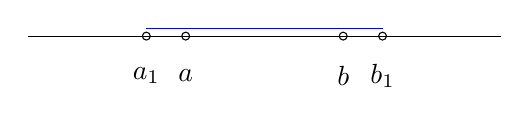
\begin{tikzpicture}
	\draw (-3,0) -- (3,0);
	\draw[blue] (-1.5,0.1) -- (1.5,0.1);
	\draw (-1,0) circle (0.05cm);
	\draw (-1,-0.5) node{$a$};
	\draw (1,0) circle (0.05cm);
	\draw (1,-0.5) node{$b$};

	\draw (-1.5,0) circle (0.05cm);
	\draw (-1.5,-0.5) node{$a_1$};
	\draw (1.5,0) circle (0.05cm);
	\draw (1.5,-0.5) node{$b_1$};
\end{tikzpicture}
\end{center}

	Suppose $b_1 < b$.
	Clearly, $a < b_1$.
	And the cover $\mathcal{C}$ must have an open interval containing $b_1$.
	Otherwise $\mathcal{C}$ is not a cover of $[a,b]$.
	That is, there exists $(a_2,b_2)$ containing $b_1 \in (a,b)$ such that $a_2 < b_1 < b_2$.
	If $b_2 > b$, then $\displaystyle \sum_{i=1}^k l(I_k) \ge l(a_1,b_1) + l(a_2,b_2) \ge l(a_1,b_2) \ge b-a$.

\begin{center}
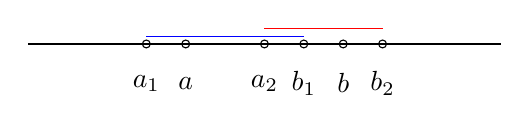
\begin{tikzpicture}
	\draw (-3,0) -- (3,0);
	\draw (-1,0) circle (0.05cm);
	\draw (-1,-0.5) node{$a$};
	\draw (1,0) circle (0.05cm);
	\draw (1,-0.5) node{$b$};

	\draw (-1.5,0) circle (0.05cm);
	\draw (-1.5,-0.5) node{$a_1$};
	\draw (0.5,0) circle (0.05cm);
	\draw (0.5,-0.5) node{$b_1$};
	\draw[blue] (-1.5,0.1) -- (0.5,0.1);

	\draw (0,0) circle (0.05cm);
	\draw (0,-0.5) node{$a_2$};
	\draw (1.5,0) circle (0.05cm);
	\draw (1.5,-0.5) node{$b_2$};
	\draw[red] (0,0.2) -- (1.5,0.2);
\end{tikzpicture}
\end{center}

	Suppose $b_2 < b$.
	Continuing like this we get, $N$ open intervals in $\mathcal{C}$, $\{ (a_k,b_k) : k = 1,2,\cdots,N \} $ such that $a_1 < a < b_1$ and $a_N < b < b_N$ and $a_k < b_{k-1} < b_k$ for all $k$.
	The process should terminate in fintie steps as $\mathcal{C}$ is a finite cover of $[a,b]$.
	Then $\displaystyle \sum_{k=1}^N l(I_k) \ge \sum_{k=1}^N l(a_k,b_k) \ge l(a_1,b_N) \ge b-a$.

\begin{center}
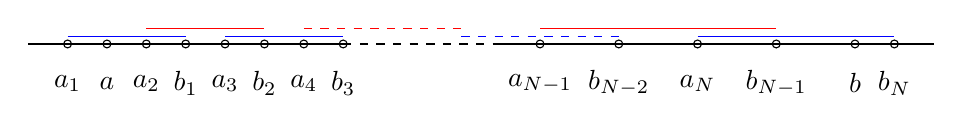
\begin{tikzpicture}
	\draw (-5,0) -- (-1,0);
	\draw[dashed] (-1,0) -- (1,0);
	\draw (1,0) -- (6.5,0);

	\draw (-4,0) circle (0.05cm);
	\draw (-4,-0.5) node{$a$};
	\draw (5.5,0) circle (0.05cm);
	\draw (5.5,-0.5) node{$b$};

	\draw (-4.5,0) circle (0.05cm);
	\draw (-4.5,-0.5) node{$a_1$};
	\draw (-3,0) circle (0.05cm);
	\draw (-3,-0.5) node{$b_1$};
	\draw[blue] (-4.5,0.1) -- (-3,0.1);

	\draw (-3.5,0) circle (0.05cm);
	\draw (-3.5,-0.5) node{$a_2$};
	\draw (-2,0) circle (0.05cm);
	\draw (-2,-0.5) node{$b_2$};
	\draw[red] (-3.5,0.2) -- (-2,0.2);

	\draw (-2.5,0) circle (0.05cm);
	\draw (-2.5,-0.5) node{$a_3$};
	\draw (-1,0) circle (0.05cm);
	\draw (-1,-0.5) node{$b_3$};
	\draw[blue] (-2.5,0.1) -- (-1,0.1);
	
	\draw (-1.5,0) circle (0.05cm);
	\draw (-1.5,-0.5) node{$a_4$};
	\draw[red,dashed] (-1.5,0.2) -- (0.5,0.2);

	\draw (2.5,0) circle (0.05cm);
	\draw (2.5,-0.5) node{$b_{N-2}$};
	\draw[blue,dashed] (0.5,0.1) -- (2.5,0.1);

	\draw (1.5,0) circle (0.05cm);
	\draw (1.5,-0.5) node{$a_{N-1}$};
	\draw (4.5,0) circle (0.05cm);
	\draw (4.5,-0.5) node{$b_{N-1}$};
	\draw[red] (1.5,0.2) -- (4.5,0.2);

	\draw (3.5,0) circle (0.05cm);
	\draw (3.5,-0.5) node{$a_N$};
	\draw (6,0) circle (0.05cm);
	\draw (6,-0.5) node{$b_N$};
	\draw[blue] (3.5,0.1) -- (6,0.1);
\end{tikzpicture}
\end{center}

	Clearly, every open cover of $[a,b]$ contains a finite subcover $\mathcal{C}$, which contains a finite subcover of the form $\{ (a_k,b_k) : k=1,2,\cdots,N \}$ such that $\displaystyle \sum_{k=1}^N l(I_k) \ge b-a$.
	Thus, for any open cover $\displaystyle \sum_{k=1}^\infty l(I_k) \ge b-a$.
	And thus,
	\begin{equation}
		m^\ast([a,b]) \ge b-a
	\end{equation}

	\textbf{Case 2 : Bounded Interval}
	Let $I$ be a bounded interval.
	Then there exists bounded closed intervals $J_1$ and $J_2$ such that $J_1 \subsetneq I \subsetneq J_2$ such that $l(I) - \epsilon < l(J_1)$ and $l(J_2) < l(I)+\epsilon$.
	Suppose $I = (a,b]$, then $J_1 = [a+\frac{\epsilon}{2}, b-\frac{\epsilon}{2}]$ and $J_2 = [a-\frac{\epsilon}{2},b+\frac{\epsilon}{2}]$.\\

	By monotonicity of Lebesgue outer measure, we have $m^\ast(J_1) \le m^\ast(I) \le m^\ast(J_2)$.
	However $m^\ast(J_1) = l(I)-\epsilon$ and $m^\ast(J_2) = l(I)+\epsilon$.
	Thus, $l(I)-\epsilon \le m^\ast(I) \le l(I)+\epsilon$.
	Therefore, $m^\ast(I) = l(I)$.

	\textbf{Case 3 : Unbounded Interval}
	Let $I$ be an unbounded interval.
	Then for any natural number $n$, there exists a closed bounded interval $J$ such that $J \subset I$ and $l(J) = n$.
	And $n = m^\ast(J) \le m^\ast(I),\ \forall n \in \mathbb{N}$.
	Therefore, $m^\ast(I) = \infty = l(I)$. 
	\end{proof}
	\item Outer Measure is translation invariant
	\begin{proof}
	Let $A$ be any set and $y \in \mathbb{R}$.
	Let $\{ I_k : k = 1,2,\dots \}$ be a cover of $A$.
	Then $\{ I_k+y : k = 1,2,\dots \}$ is a cover of $A+y$.
	And $l(I_k) = l(I_k+y)$ for every natural number $k$ and real number $y$.
	Thus, $\displaystyle \sum_{k=1}^\infty l(I_k) = \sum_{k=1}^\infty l(I_k+y)$.
	Clearly, for each cover $\{I_k\}_{k=1}^\infty$ of $A$, there exists a cover $\{ I_k+y \}_{k=1}^\infty$ of $A+y$ containing intevals of same length.
	Therefore, $m^\ast(A) = m^\ast(A+y)$.
	\end{proof}
	\item Outer Measure is countably subadditive
	\begin{proof}
	Let $\{E_k\}_{k=1}^\infty$ be a countable collection of sets.
	It is enough to prove that
		\begin{equation}
			m^\ast \left( \bigcup_{k=1}^\infty E_k \right) \le \sum_{k=1}^\infty m^\ast(E_k)
		\end{equation}
		For each natural number $k$, we have a cover of $E_k$, say $\{ I_{k,i} \}_{i = 1}^\infty$ such that $\displaystyle \sum_{i=1}^\infty I_{k,i} < m^\ast(E_k) + \frac{\epsilon}{2^k}$.
		Suppose that, for some $\epsilon > 0$, $E_k$ doesn't have such a cover, then $m^\ast(E_k) + \frac{\epsilon}{2^k}$ is an upper bound contradicting the assumption that $m^\ast(E_k)$ is the least upper bound.\\

	Clearly,
	\begin{align*}
		m^\ast \left( \bigcup_{i,k = 0}^\infty I_{k,i} \right) \le & \sum_{k=1}^\infty \sum_{i=1}^\infty I_{k,i} \\
		= & \sum_{k=1}^\infty \left( m^\ast(E_k) + \frac{\epsilon}{2^k} \right) \\
		= & \sum_{k=1}^\infty  m^\ast(E_k) + \epsilon
	\end{align*}
	\end{proof}
	\textbf{Note : } Finite subadditivity is a weaker notion than countable subadditivity.
	Since every finite collection is a countable collection.
\end{enumerate}

\subsubsection{Exercise}
\begin{enumerate}
	\setcounter{enumi}{4}
\item Closed Interval $[0,1]$ is uncountable.\\
	Suppose $[0,1]$ is countable, then Lebesgue outer measure of any countable set is zero, $m^\ast([0,1]) = 0$.
		But, $[0,1]$ is an interval and Lebesgue outer measure of an interval is its length, $m^\ast([0,1]) = l([0,1]) = 1$ which is a contradiction.
\item $m^\ast([0,1] - \mathbb{Q}) = 1$
	$$[0,1] = \left( [0,1] \cap \mathbb{Q} \right)\ \cup\ \left( [0,1]\cap \mathbb{Q}^c \right)$$
	Clearly, $m^\ast([0,1]) = 1$.
		And $[0,1] \cap \mathbb{Q}$ is a countable set since $\mathbb{Q}$ is countable.
		And thus has Lebesgue outer measure zero.
		Thus by countable subadditivity, we have
	$$1 = m^\ast([0,1]) \le m^\ast([0,1] \cap \mathbb{Q}^c) + 0$$
		Thus, $m^\ast([0,1] \cap \mathbb{Q}^c) \ge 1$.
		And $[0,1] \cap \mathbb{Q}^c\ \subset [0,1]$.
		By monotonicity, $m^\ast([0,1] \cap \mathbb{Q}^c) \le m^\ast([0,1]) = 1$.
		Therefore, $m^\ast([0,1] \cap \mathbb{Q}^c) = 1$.
	\item Construction of a $G_\delta$ set containing $E$ % hint : $G_\delta = \cup_{k=1}^\infty F_k$ where
	\item hint : if sum of interval is less than 1.
		Then it is not a cover of $[0,1]$.
	\item hint : $A \cup B = A \cup (B-A) = A \cup (B \cap A^c)$
	\item hint : $A$ and $B$ are separated by distance $\alpha$, thus are disjont.
\end{enumerate}

\subsection{$\sigma$-algebra of Lebesgue Measurable Sets}
	Lebesgue Outer Measure is defined for any subset of real numbers and Lebesgue outer measure of an interval is its length.
	However, it isn't countable additive.\\

	There exists disjoint sets $A,B$ such that $m^\ast(A\cup B) < m^\ast(A)+m^\ast(B)$.\\
	
	Since countable additivity is a favourable property over countable subadditivity.
	We restrict the family of subsets of real numbers to those subsets that allow countable additivity.
	
\subsubsection{Lebesgue Measurable Set}
\begin{definition}[Measurable Set]
	Let $E$ be a subset of $\mathbb{R}$.
	Then $E$ is Lebesgue measurable if
\begin{equation}
	m^\ast(A) = m^\ast(A \cap E) + m^\ast(A \cap E^c)
	\label{eq:measurable1}
\end{equation}
	for any subset $A$ of $\mathbb{R}$.
\end{definition}

	In other words, $E$ is Lebesgue measurable if $E$ doesn't affect countable additivity of Lebesgue Outer Measure.\\

	We will consider only those subset of real numbers, which won't affect countable additivity.
	These subsets are \textbf{Lebesgue Measurable}.
	And we could show that the collection of all Lebesgue Measurable sets forms a $\sigma$-algebra.
	Clearly, intervals allow countable additivity, thus the Borel Algebra is contained in this $\sigma$-algebra of Lebesgue measurable sets.
\subsubsection{Simplified Condition for Lebesgue Measurability}

We know that Lebesgue Outer Measure has countable subadditivity.
\begin{equation*}
	m^\ast(A) \le m^\ast(A \cap E) + m^\ast(A \cap E^c)
\end{equation*}
Thus, for condition (\ref{eq:measurable1}), it is sufficient to check the following condition,
\begin{equation}
	m^\ast(A) \ge m^\ast(A \cap E) + m^\ast(A \cap E^c)
	\label{eq:measurable2}
\end{equation}

\subsubsection{Properties of Lebesgue Measure}
\begin{enumerate}
	\item Any set of Lebesgue outer measure zero is Lebesgue measurable.
	\begin{proof}
		Let $E$ be a subset of real numbers with Lebesgue outer measure zero.
		Let $A$ be any subset of real numbers.
		Then $A = (A \cap E) \cup (A \cap E^c)$.
		By countable additivity, $m^\ast(A) \le m^\ast(A \cap E) + m^\ast(A \cap E^c)$.
		Since $A\cap E \subset E$, we have by monotonicity $m^\ast(A \cap E) \le m^\ast(E) = 0$.\\


		Again, $A \cap E^c \subset A$ and by monotonicity, $m^\ast(A) \ge m^\ast(A \cap E^c) = 0+m^\ast(A \cap E^c) = m^\ast(A\cap E) + m^\ast(A \cap E^c)$.
		Thus, $E$ is Lebesgue measurable by the simplified condition for Lebesgue measurability.
	\end{proof}

	\item Countable sets are Lebesgue measurable.
	\begin{proof}
	Countable sets are of Lebesgue outer measure zero.
	And sets of Lebesgue outer measure zero are Lebesgue measurable.
	Thus, they are Lebesgue measurable.
	\end{proof}
	\item Finite union of Lebesgue measurable sets is Lebesgue measurable.
	\begin{proof}
		It is enough to prove that if $E_1$ and $E_2$ are Lebesgue measurable, then their union is also Lebesgue measurable.
		Then, by finite mathematical induction, we can prove that the result if true for any finite collection of Lebesgue measurable sets.\\


	Suppose $E_1, E_2$ are Lebesgue measurable sets.
	Since $E_1$ is Lebesgue measurable,
	\begin{equation}
		m^\ast(A) = m^\ast(A \cap E_1) + m^\ast(A \cap E_1^c)
	\end{equation}
	And consider $A \cap E_1^c$ instead of $A$.
	Since $E_2$ is Lebesgue measurable, we get
	\begin{equation}
		m^\ast(A \cap E_1^c) = m^\ast(A \cap E_1^c\cap  E_2) + m^\ast(A \cap E_1^c \cap E_2^c)
	\end{equation}

	We have $(A \cap E_1^c) \cap E_2^c = A \cap (E_1^c \cap E_2^c) = A \cap (E_1 \cup E_2)^c$.
	And $(A \cap E_1) \cup (A \cap E_1^c \cap E_2) = (A \cap E_1) \cup [A \cap (E_2 \cap E_1^c)] = A \cap (E_1 \cup E_2)$.
\begin{center}
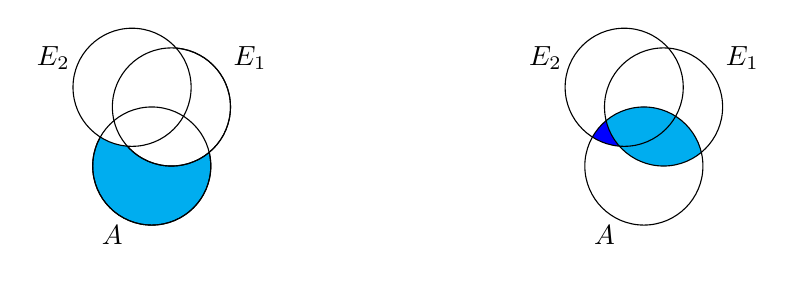
\begin{tikzpicture}[scale=0.25]
	\filldraw[fill = cyan] (0,-1.5) circle (3cm);
	\filldraw[fill = white] (1,1.5) circle (3cm);
	\filldraw[fill = white] (-1,2.5) circle (3cm);
	\draw (0,-1.5) circle (3cm);
	\draw (1,1.5) circle (3cm);
	\draw (-2,-5) node{$A$};
	\draw (5,4) node{$E_1$};
	\draw (-5,4) node{$E_2$};

	\begin{scope}
		\clip (25,-1.5) circle (3cm);
		\fill[blue] (24,2.5) circle (3cm);
	\end{scope}
	\begin{scope}
		\clip (25,-1.5) circle (3cm);
		\fill[cyan] (26,1.5) circle (3cm);
	\end{scope}
	\draw (25,-1.5) circle (3cm);
	\draw (26,1.5) circle (3cm);
	\draw (24,2.5) circle (3cm);
	\draw (23,-5) node{$A$};
	\draw (30,4) node{$E_1$};
	\draw (20,4) node{$E_2$};
\end{tikzpicture}
\end{center}
	\begin{align*}
		m^\ast(A) = & m^\ast(A \cap E_1) + m^\ast(A \cap E_1^c) \\
		= & {\color{blue}m^\ast(A \cap E_1) + m^\ast(A \cap E_1^c \cap E_2)} + m^\ast(A \cap E_1^c \cap E_2^c) \\
		\ge & {\color{blue}m^\ast[A \cap (E_1 \cup E_2)]} + m^\ast[A \cap (E_1 \cup E_2)^c] 
	\end{align*}
	Therefore $E_1 \cup E_2$ is Lebesgue measurable.
		And by finite induction, finite union of Lebesgue measurable sets is also Lebesgue measurable.
	\end{proof}

	\item Lebesgue Measure is finitely additive.\\
		In other words, Suppose $\{E_k\}_{k = 1}^n$ be a finite collection of disjoint, Lebesgue measurable sets.
		Then Lebesgue measure of their union is the sum of Lebesgue measures.
	\begin{proof}
	Let $A$ be any subset of $\mathbb{R}$ and $\{ E_k \}_{k=1}^n$ be a finite collection of disjoint, Lebesgue measurable subsets of $\mathbb{R}$.
	\begin{equation}
		\text{Claim : }	m^\ast \left( A \cap \left[ \bigcup_{k=1}^\infty E_k\right] \right) = \sum_{k=1}^\infty m^\ast (A \cap E_k)
	\end{equation}
	Trivially, the claim is true for $n=1$.
		Suppose the claim is true for $n-1$.
		That is,
	\begin{equation}
		m^\ast \left( A \cap \left[ \bigcup_{k=1}^{n-1} E_k \right] \right) = \sum_{k=1}^{n-1} m^\ast (A \cap E_k)
	\end{equation}
	From set theory we have,
	\begin{align}
		A \cap \left[ \bigcup_{k=1}^n E_k \right] \cap E_n & = A \cap E_n\\
		A \cap \left[ \bigcup_{k=1}^n E_k \right] \cap E_n^c  & = A \cap \left[ \bigcup_{k=1}^{n-1} E_n \right]
	\end{align}
	By Lebesgue measurability of $E_n$, we have
	\begin{align*}
		m^\ast \left( A \cap \left[ \bigcup_{k=1}^n E_k \right] \right) = & m^\ast \left( A \cap \left[ \bigcup_{k=1}^n E_k \right] \cap E_n \right) + m^\ast \left( A \cap \left[ \bigcup_{k=1}^n E_k \right] \cap E_n^c \right)\\
		& = m^\ast \left( A \cap E_n \right) + m^\ast  \left( A \cap \left[ \bigcup_{k=1}^{n-1} E_n \right] \right) \\
		& =  \sum_{k=1}^n m^\ast \left( A \cap E_k \right) \text{, by mathematical induction}
	\end{align*}
	Taking $A = \mathbb{R}$, we get Lebesgue measure is finitely additive.
		That is,
	\begin{equation}
		m^\ast \left( \bigcup_{k=1}^n E_k \right) = \sum_{k=1}^n m^\ast \left( E_k \right)
	\end{equation}
	\end{proof}
\item Countable union of Lebesgue measurable sets is Lebesgue measurable
	\begin{proof}
		Let $A$ be any subset of $\mathbb{R}$.
		And $\{ E_k \}_{k=1}^\infty$ be a countable collection of disjoint, Lebesgue measurable subsets of $\mathbb{R}$.
		Define $F_n = \cup_{k=1}^n E_k$ and $E = \cup_{k=1}^\infty E_k$.
		Clearly, $F \subset E$ and $F^c \supset E^c$.
		Thus, $m^\ast(A \cap F_n^c) \ge m^\ast(A \cap E^c)$.
	\begin{align*}
		m^\ast(A) & =  m^\ast (A \cap F_n) + m^\ast (A \cap F_n^c) \\
		& \ge m^\ast \left( A \cap \left[ \bigcup_{k=1}^n E_k \right] \right) + m^\ast(A \cap E^c) \\
		& \ge \sum_{k=1}^n m^\ast(A \cap E_k) + m^\ast(A \cap E^c) 
	\end{align*}
	\begin{align*}
		\lim_{n \to \infty} m^\ast(A) & \ge \lim_{n \to \infty} \sum_{k=1}^n m^\ast(A \cap E_k) + m^\ast(A \cap E^c) \\
		m^\ast(A) & \ge \sum_{k=1}^\infty m^\ast(A \cap E_k) + m^\ast (A \cap E^c) \\
		& \ge m^\ast \left( A \cap \left[ \bigcup_{k=1}^\infty E_k \right] \right) + m^\ast(A \cap E^c) \\
		\implies m^\ast(A) & \ge m^\ast (A \cap E) + m^\ast(A \cap E^c)
	\end{align*}
		By above inequality, $E = \cup_{k=1}^\infty E_k$ is Lebesgue measurable.\\

		And, any countable collection of Lebesgue measurable sets can be expressed as a countable collection of disjoint, Lebesgue measurable sets.
		Let $\{ E_k \}_{k=1}^\infty$ be a collection of Lebesgue measurable sets.
		Then, the countable collection, $\{ E_k' \}_{k=1}^\infty$ defined by $E_k'= E_k - \cup_{j=1}^{k-1}E_k$ contains disjoint, Lebesgue measurable\dag\footnote{
			Suppose $E_1,E_2$ are measurable, then $E_2^c = \mathbb{R} - E_2$ is measurable by the duality of measurability condition.
		And $E_1 \cap E_2^c = E_1-E_2$ is Lebesgue measurable since countable intersection of Lebesgue measurable sets is Lebesgue measurable (by Property 4 and de Morgan's Law).}
	subsets of $\mathbb{R}$.
		Therefore, countable union of Lebesgue measurable sets is Lebesgue measurable.
	\end{proof}
	\item Every interval is Lebesgue measurable.
	\begin{proof}
	It is sufficient to prove that $(a,\infty)$ is Lebesgue measurable.
	Suppose $(a,\infty)$ is Lebesgue measurable for every $a \in \mathbb{R}$.
	Then interval $(a,b)$ is Lebesgue measurable, since $(a,b) = [(a,\infty) \cap (\mathbb{R}-(b,\infty))]-\{b\}$.\\


	Let $A$ be any subset of $\mathbb{R}$.
	Define $A_1 = A\cap (-\infty,a)$ and $A_2 = A \cap (a,\infty)$ such that $A-\{a\} = A_1 \cup A_2$ and $A_1 \cap A_2 = \phi$.
	And the interval $(a,\infty)$ is Lebesuge measurable only if 
	\begin{equation}
		m^\ast(A) \ge m^\ast(A \cap (a,\infty)) + m^\ast(A \cap (a,\infty)^c) = m^\ast(A_1)+m^\ast(A_2)
		\dag\footnote{We have, $m^\ast(A \cap (-\infty,a]) = m^\ast(A \cap (-\infty,a)$ since removing finite number of points from a subset of $\mathbb{R}$ won't affect its Lebesgue measure.}
	\end{equation}
	Let collection $\{ I_k \}_{k=1}^\infty$ be a countable cover of $A$.
		Then collection $\{ I_k' \}_{k=1}^\infty$ defined by $I_k' = I_k \cap (a,\infty)$ is a cover of $A_1$.
		And collection $\{I_k''\}_{k=1}^\infty$ defined by $I_k'' = I_k \cap (-\infty,a)$ is a cover of $A_2$.\\

	Clearly, $\displaystyle m^\ast(A_1) \le \sum_{k=1}^\infty l(I_k')$ and $\displaystyle m^\ast(A_2) \le \sum_{k=1}^\infty l(I_k'')$.
	\begin{align*}
		m^\ast(A_1)+m^\ast(A_2) & \le \sum_{k=1}^\infty l(I_k') + \sum_{k=1}^\infty l(I_k'') \\
		& \le \sum_{k=1}^\infty l(I_k') + l(I_k'') \\
		& \le \sum_{k=1}^\infty l(I_k) \le m^\ast(A)
	\end{align*}
		Thus, $(a,\infty)$ is Lebesgue measurable.
		Therefore, every interval is Lebesgue measurable.
	\end{proof}
	\item $\sigma$-algebra of Lebesgue measurable sets $\mathcal{M}$ contains Borel Sets $\mathcal{B}$.
	\begin{equation}
		\mathcal{B} \subset \mathcal{M}
	\end{equation}
	\begin{proof}
	The Borel algebra $\mathcal{B}$ is the $\sigma$-algebra containing all intervals.
		We have proved that, every intervals are Lebesgue measurable.
		Also, we have proved that the set of all Lebesgue measurable subsets of $\mathbb{R}$ is a $\sigma$-algebra as complements of Lebesgue measurable sets are Lebesgue measurable by duality of the condition and countable union of Lebesgue measurable sets are also Lebesgue measurable.
		Therefore, every Borel set is Lebesgue measurable.
		Clearly, $G_\delta$ and $F_\sigma$ are Borel sets and are Lebesgue measurable.
	\end{proof}
	\item Lebesgue Measurability is translation invariant.
	\begin{proof}
		Let $E$ be a Lebesgue measurable set.
		Let $A$ be any subset of $\mathbb{R}$ and $y \in \mathbb{R}$.
		Then,
	\begin{align*}
		m^\ast(A) & = m^\ast(A-y)\\
		& = m^\ast((A-y) \cap E) + m^\ast((A-y) \cap E^c)\\
		& = m^\ast(A \cap (E+y)) + m^\ast(A \cap (E+y)^c)
	\end{align*}
		Thus, $E+y$ is Lebesgue measurable.
		And Lebesgue measurability is traslation invariant.
	\end{proof}
\end{enumerate}

\subsubsection{Exercise}
\begin{enumerate}
	\setcounter{enumi}{10}
	\item Let $\mathcal{A}$ be the $\sigma$-algebra containing all intervals of the form $(a, \infty)$.
		Every interval has one of the four forms,
	\begin{align}
		(a,b] = & (a,\infty) \cap (b,\infty)^c \\
		(a,b) = & (a,\infty) \cap \left[\bigcap_{k=1}^\infty \left(b-\frac{1}{k},\infty\right)\right]^c \\
		[a,b] = & \left[ \bigcap_{k=1}^\infty \left(a-\frac{1}{k},\infty\right)\right] \cap (b,\infty)^c \\
		[a,b) = & \left[\bigcap_{k=1}^\infty \left(a-\frac{1}{k},\infty\right)\right] \cap \left[ \bigcap_{k=1}^\infty \left(b-\frac{1}{k},\infty\right)\right]^c
	\end{align}
\item \textbf{Borel sets} is the $\sigma$-algebra containing all open intervals.
	The equations from previous equations are sufficient.
	However, we have a simpler form for closed intervals, $[a,b]$.
	\begin{align}
		[a,b] = & \left[(-\infty,a) \cup (b,\infty) \right]^c 
	\end{align}
		Clearly, every interval is a Borel set.
	\item
	\begin{itemize}
		\item $C \in F_\sigma \implies C = \bigcup_{k=1}^\infty C_k \implies \bigcup_{k=1}^\infty \left(C_k+y\right) = C+y \in F_\sigma$
		\item $O \in G_\delta \implies O = \bigcap_{k=1}^\infty O_k \implies \bigcup_{k=1}^\infty \left( O_k+y \right) =  O+y \in G_\delta$
		\item $m^\ast(E) = 0 \implies 0 = \inf\{\sum_{k=1}^\infty l(I_k)\} = \inf\{\sum_{k=1}^\infty l(I_k+y)\} \implies  m^\ast(E+y) = 0$
	\end{itemize}
	\item A subset $E$ has positive Lebesgue measure if and only if it has a bounded subset of positive Lebesgue measure.
		$$m^\ast(E) > 0 \iff \exists \text{ bounded subset }F \subset E,\text{ such that } m^\ast(F) > 0$$
		\textbf{Sufficient Part :} By monotonicity, $F \subset E \implies m^\ast(F) \le m^\ast(E)$.
		And $m^\ast(F) > 0 \implies 0 < m^\ast(F) \le m^\ast(E)$.\\
		\textbf{Necessary Part :}
	\item 
\end{enumerate}

\subsection{Outer and Inner Approximation}
\begin{definition}[Excision Property]
Let $A$ be a Lebesgue measurable set of finite measure and $A \subset B$.
	Then,
\begin{equation}
	m^\ast(B \sim A) = m^\ast(B) - m^\ast(A)
\end{equation}
\begin{proof}
\begin{align*}
	m^\ast(B) = & m^\ast(B \cap A) + m^\ast(B \cap A^c) \\
	= & m^\ast(A) + m^\ast(B \sim A) \\
	\implies m^\ast(B \sim A) = & m^\ast(B) - m^\ast(A)
\end{align*}
\end{proof}
\end{definition}

\begin{theorem}[approximation]
	The following conditions are equivalent to Lebesgue measurability of $E$
\begin{enumerate}
	\item $\forall \epsilon > 0$, there is an open set $\mathcal{O}$ containing $E$ for which $m^\ast(\mathcal{O}\sim E) < \epsilon$.
	\item There is a $G_\delta$ set $G$ containining $E$ such that $m^\ast(G \sim E) = 0$.
	\item $\forall \epsilon > 0$, there is a closed set $F$ contained in $E$ such that $m^\ast(E\sim F) = 0$.
	\item There is an $F_\sigma$ set $F$ contained in $E$ sucht hat $m^\ast(E \sim F) = 0$.
\end{enumerate}
\end{theorem}

\textbf{Note :} Equivalent conditions 1 \& 2 are about outer approximation of a Lebesgue measurable set and 3 \& 4 are about inner approximation of a Lebesgue measurable set.\\

\begin{proof}
\subsubsection*{Measurability $\implies$ Open set - Outer approximation}
	Suppose that $E$ is Lebesgue measurable.
	And let $\epsilon > 0$.\\


	\textbf{Case 1 :} Suppose $m^\ast(E) < \infty$.
	By definition of Lebesgue outer measure, there exists an open cover $\{ I_k \}_{k=1}^\infty$ such that $\displaystyle \sum_{k=1}^\infty l(I_k) <  m^\ast(E)+\epsilon$.\\

	Define $\mathcal{O} = \displaystyle \bigcup_{k=1}^\infty I_k$.
	Then $\mathcal{O}$ is an open set containing $E$ and thus Lebesgue measurable.
	Also, $\displaystyle m^\ast(\mathcal{O}) \le \sum_{k=1}^\infty l(I_k) < m^\ast(E) + \epsilon$.
	Therefore, by excision property we have $m^\ast(\mathcal{O} \sim E) = m^\ast(\mathcal{O}) - m^\ast(E) < \epsilon$. \\

	\textbf{Case 2 :} Suppose $m^\ast(E) = \infty$.
	Without loss of generality, $E$ may be written as countable union Lebesgue measurable sets $\{ E_k \}_{k=1}^\infty$ of finite measure.\\

	By case 1, for every $k$, there exists $\mathcal{O}_k$ for each $E_k$ of finite measure such that $m^\ast(\mathcal{O}_k \sim E_k) < \frac{\epsilon}{2^k}$.
	Define $\displaystyle \mathcal{O} = \bigcup_{k=1}^\infty \mathcal{O}_k$.
	Then $\mathcal{O}$ is open, contains $E$ and 
	\begin{align*}
		m^\ast(\mathcal{O} \sim E) = & m^\ast\left(\bigcup_{k=1}^\infty \mathcal{O}_k \sim E \right) \\
		\le & m^\ast \left(\bigcup_{k=1}^\infty \mathcal{O}_k \sim E_k \right) \\
		\le & \sum_{k=1}^\infty m^\ast(\mathcal{O}_k \sim E_k) = \epsilon \sum_{k=1}^\infty \frac{1}{2^k} = \epsilon
	\end{align*}

\subsubsection*{Open, Outer approximation $\implies G_\delta$, Outer approximation }
	Let $E$ be a subset of real numbers such that Lebesgue measure of $E$ has an open set inner approximation.
	That is, for every $\epsilon > 0$, there exits an open set $\mathcal{O}$ such that $m^\ast(\mathcal{O} \sim E) < \epsilon$.\\

	Let $\mathcal{O}_k$ be open sets such that $m^\ast(\mathcal{O}_k \sim E) < \frac{1}{k}$.
	Define $\displaystyle G = \bigcap_{k=1}^\infty \mathcal{O}_k$.
	Then, $G$ is a $G_\delta$ set containing $E$.
	And $G \sim E \subset \mathcal{O}_k \sim E$.
	Thus, by monotonicity, $m^\ast(G \sim E) \le m^\ast(\mathcal{O}_k \sim E) < \frac{1}{k}$.
	Thus, we have a $G_\delta$ set $G$ containing $E$ such that $m^\ast(G \sim E) = 0$.

\subsubsection*{$G_\delta$-Outer approximation $\implies$ Measurability}
	We have, $m^\ast(G \sim  E) = 0$.
	Since every set of Lebesgue measure zero is Lebesgue measurable, $G \sim E$ is Lebesgue measurable.
	And its complement $(G \sim E)^c$ is also Lebesgue measurable.
	Also we have, $G$ is a $G_\delta$ set, thus a Borel set and hence Lebesgue measurable.\\

	Clearly,we have $E = G \cap (G \sim E)^c$.
	And therefore, $E$ is Lebesgue measurable.

\subsubsection*{Open, Outer approximation $\iff$ Closed, Inner approximation}
	By duality of Lebesgue measurability, $E$ is Lebesgue measurable if and only if $E^c$ is Lebesgue measurable.
	And by de Morgan's Law, we have $E^c$ has an open set - outer approximation $\mathcal{O}$ if and only if $E$ has a closed set - inner approximation $\mathcal{O}^c$.
	$$ m^\ast(\mathcal{O} \sim E^c) < \epsilon \iff m^\ast(E \sim \mathcal{O}^c) < \epsilon $$

\subsubsection*{$G_\delta$-Outer approximation $\iff F_\sigma$-Inner approximation}
	Again, by duality of Lebesgue measurability and de Morgan's Law, we have $E^c$ has a $G_\delta$-outer approximation $G$ if and only if $E$ has an $F_\sigma$-inner approximation $F$.
	$$ m^\ast(G \sim E^c) < \epsilon \iff m^\ast(E \sim F) < \epsilon $$
\end{proof}

\begin{theorem}
	Let $E$ be a Lebesgue measurable set of finite measure.
	Then for any $\epsilon > 0$, there exists a finite collection of disjoint open sets $\{ I_k \}_{k=1}^n$ such that  $\displaystyle \mathcal{O} = \bigcup_{k=1}^n I_k$ and $m^\ast(\mathcal{O} \sim E) + m^\ast(E-\mathcal{O}) < \epsilon$.
\end{theorem}
\begin{proof}
	Since $E$ is Lebesgue measurable, by outer approximation theorem we have an open set $U$ such that $E \subset U$ and 
	\begin{equation*}
		m^\ast(U \sim E) < \frac{\epsilon}{2}
	\end{equation*}

	\begin{align*}
		U =  & (U \cap E) \cup (U \cap E^c)
		\intertext{Since $E$ is Lebesgue measurable, $m^\ast(E) < k$}
		m^\ast(U) = &  m^\ast(U \cap E) + m^\ast(U \cap E^c) \\
		= & m^\ast(E) + m^\ast(U \sim E)
		\intertext{Since $E$ has finite measure}
		m^\ast(U) = & m^\ast(E) + m^\ast(U \sim E) \\
		< & k+\frac{\epsilon}{2} < \infty
	\end{align*}
	That is, $U$ is of finite measure. \\

	Since $U$ is open, $U$ is countable\dag\footnote{
		By definition, \textbf{Open sets} are countable union of disjoint, open intervals}
	union of a disjoint collection of open intervals, say $\{ I_k \}_{k=1}^\infty$. Clearly,
	\begin{align*}
		\sum_{k=1}^n l(I_k) & \le \sum_{k=1}^\infty \le m^\ast(U) < \infty \\
		\sum_{k=1}^\infty l(I_k) & < \infty 
		\intertext{ By characterisation of series convergence, there exists an integer $n$ such that,}
		\sum_{k=n+1}^\infty l(I_k) & < \frac{\epsilon}{2}
	\end{align*}
	Define $\displaystyle \mathcal{O} = \bigcup_{k=1}^n I_k$.
	Since $\mathcal{O} \sim E \subset U \sim E$, by monotonicity we have 
	\begin{equation}
		m^\ast(\mathcal{O} \sim E) \le m^\ast(U \sim E) < \frac{\epsilon}{2}
	\end{equation}

	Since $E \subset U$, we have $\displaystyle E \sim \mathcal{O} \subset U \sim \mathcal{O} = \bigcup_{k=1}^n I_k$.
	And clearly, 
	\begin{equation*} 
		U \sim \mathcal{O} = \bigcup_{k=1}^\infty I_k \sim \bigcup_{k=1}^n I_k = \bigcup_{k=n+1}^\infty I_k
	\end{equation*}
	\begin{align}
		\text{Thus, } m^\ast(E \sim \mathcal{O}) \le & m^\ast(U \sim \mathcal{O}) \le \sum_{k=n+1}^\infty l(I_k) < \frac{\epsilon}{2} 
		\intertext{Therefore,}
		m^\ast(E \sim \mathcal{O}) + m^\ast(\mathcal{O} \sim E) < & \epsilon \nonumber
	\end{align}
\end{proof}

\subsubsection{Exercise}

\begin{enumerate}
	\setcounter{enumi}{16}
\item Let $\epsilon > 0$ and $E$ is Lebesgue measurable.
	Then there exists open set $\mathcal{O}$ and closed set $F$ such that $F \subset E \subset \mathcal{O}$, $m^\ast(E \sim F) < \frac{\epsilon}{2}$ and $m^\ast(\mathcal{O} \sim E) < \frac{\epsilon}{2}$.
	Clearly, $\mathcal{O} \sim E$ and $E \sim F$ are disjoint and $\mathcal{O} \sim F = (\mathcal{O} \sim E) \cup (E \sim F)$.
		Thus by monotonicity of Lebesgue outer measure, we have $m^\ast(\mathcal{O} \sim F) \le m^\ast(\mathcal{O} \sim E) + m^\ast(E \sim F) < \epsilon$.
\item
 Suppose $E$ has finite outer measure.
	\dag\footnote{
		$E$ has finite outer measure does not imply $E$ is bounded or Lebesgue measurable.}\\
	\textbf{$G_\delta$ set : }
	Let $\epsilon > 0$.
	Then by the definition of Lebesgue outer measure, there exists a cover $\{ I_k \}_{k=1}^\infty$ of $E$ such that $\displaystyle \sum_{k=1}^\infty l(I_k) < m^\ast(E) - \frac{\epsilon}{2}$.
	Define $\displaystyle G = \bigcup_{k=1}^\infty I_k$.
	Then $G$ is a $G_\delta$ set and $\displaystyle m^\ast(G) \le \sum_{k=1}^\infty l(I_k) < m^\ast(E) - \frac{\epsilon}{2}$.\\

	\textbf{$F_\sigma$ set : }
		%---yet to update---
\item
 	Let $E$ be a set of finite outer measure.
	Suppose $E$ is not Lebesgue measurable.
	And $\mathcal{O}$ be an open set containing $E$.
	Then $\mathcal{O} = (\mathcal{O} \sim E) \cup E$.
		By monotonicity, $m^\ast(\mathcal{O}) \textcolor{red}{ \le } m^\ast(\mathcal{O} \sim E) + m^\ast(E)$
		\dag\footnote{\textcolor{red}{I am not able to change $\le$ into $<$} as non-measurability doesn't mean that for this particular $\mathcal{O}$ the sum of Lebesgue outer measures should be greater. There may be a better proof.}.
	Since $m^\ast(E)$ is finite, we have $m^\ast(\mathcal{O}) - m^\ast(E) \le m^\ast(\mathcal{O} \sim E)$.
\item  Let $E$ be a set of finite outer measure.
	Suppose $E$ is Lebesgue measurable.
	Let $(a,b)$ be any open, bounded interval.
	Then by the definiton of Lebesgue measurability, $b-a = m^\ast(a,b) = m^\ast((a,b) \cap E) + m^\ast((a,b) \cap E^c)$.
%	Suppose $m^\ast(\mathcal{O}) = m^\ast(\mathcal{O} \cap E) + m^\ast(\mathcal{O} \cap E^c)$ for every open, bounded interval $\mathcal{O}$.
\item  
 	A subet $E$ is Lebesgue measurable if there exists a $G_\delta$ set $G$ containing $E$ such that $m^\ast(G \sim E) = 0$.
	Suppose $E_1$ and $E_2$ are Lebesgue measurable sets.	
	Then, we have $G_\delta$ sets $G_1$ and $G_2$.
	And two countable family of open intervals $\{\mathcal{O}_{1,k}\}_{k=1}^\infty$ and $\{ \mathcal{O}_{2,k}\}_{k=1}^\infty$ such that $\cap \mathcal{O}_{1,k} = G_1$ and $\cap \mathcal{O}_{2,k} = G_2$.
	Let $\mathcal{O} = \{ \mathcal{O}_k \}_{k=1}^\infty$ be collection of open intervals in $\mathcal{O}_1$ and $\mathcal{O}_2$.
	Define $G = \cap_{k=1}^\infty \mathcal{O}_k$.
	Then, $E = E_1 \cup E_2 \subset G_1 \cup G_2 = G$.
	Since $G \sim E = (G_1 \sim E_1) \cup (G_2 \cup E_2)$, by monotonicity of Lebesgue outer measure we have $m^\ast(G \sim E) \le m^\ast(G_1 \sim E_1) + m^\ast(G_2 \sim E_2) = 0$.
\item
	Let $m^{\ast\ast}$ be a non-negative set function defined by $m^{\ast\ast}(A) = \inf \{ m^\ast(\mathcal{O}) : A \subset \mathcal{O}, \mathcal{O} \text{ is open} \}$.
	Suppose $E$ is Lebesgue measurable.
	Then, by open set - outer approximation theorem
	we have $m^\ast(E) \le m^{\ast\ast}(E) < m^\ast(E) + \epsilon$ for any $\epsilon > 0$.
	Thus, $m^{\ast\ast}(E) = m^\ast(E)$. \\

	In other words, for Lebesgue measurable sets $m^\ast$ and $m^{\ast\ast}$ are the same.
\item  
	Let $m^{\ast\ast\ast}$ be a non-negative set function defined by $m^{\ast\ast\ast}(E) = \sup \{ m^\ast(F) : F \subset E, F \text{ is closed } \}$.
	Let $E$ be Lebesgue measurable set.
	Then, by closed set - inner approximation theorem
	we have $m^\ast(E) \ge m^{\ast\ast\ast}(E) > m^\ast(E)-\epsilon$.\\

	In other words, for Lebesgue measurable sets $m^\ast$ and $m^{\ast\ast\ast}$ are the same.
\end{enumerate}
\subsection{Further Properties}
	The Lebesgue measure has the following properties.
	\begin{enumerate}
		\item Every Borel set is Lebesgue measurable.
		\item Lebesgue Measure of an interval is its length.
		\item Lebesuge Measure is translation invariant.
		\item Lebesuge Measure is countably additive.
		\item There exists non-measurable(Lebesgue) sets. eg. $C_E \subset E$
		\item There exists uncountable set of zero measure. eg. Cantor set
	\end{enumerate}
\subsubsection{Countable Subadditivity}
\begin{theorem}
	The set function Lebesgue measure defined on $\sigma$ algebra of Lebesgue measurable sets
	\begin{enumerate*}
		\item assigns length to any interval, 
		\item is translation invariant, and
		\item is countably additive.
	\end{enumerate*}
\end{theorem}
\begin{proof}
\textbf{Length of interval}\\
	Let $E$ be an interval, then $E$ belongs to the $\sigma$ algebra of Lebesgue measurable sets as Borel sets are Lebesgue measurable.
	Also, we have $m^\ast(E) = m(E)$ for any Lebesgue measurable set $E$.
	And Lebesgue outer measure $m^\ast$ of an interval is its length.
	Therefore, Lebesgue measure of any interval is its length.\\

	\textbf{Translation invariant}\\
	Let $E$ be a Lebesgue measurable set.
	We have, $E+y$ is also Lebesgue measurable.
	Since $E+y$ is Lebesgue measurable and Lebesgue outer measure is translation invariant, we have $m^\ast(E) = m^\ast(E+y) = m(E+y)$.
	Clearly, $m(E) = m(E+y)$.\\

	\textbf{Countably additive}
	\footnote{ A real-valued set function $m$ is countably additive if $m(\cup_{k=1}^\infty E_k) = \sum_{k=1}^\infty m(E_k)$ for any disjoint family of sets $\{E_k\}$.}\\
	Let $\{ E_k \}_{k=1}^\infty$ be a countable family of disjoint, Lebesgue measurable sets.
	Lebesgue outer measure is countably subadditive and countable union of Lebesgue measurable sets is also Lebesgue measurable.
	Thus we have,
	\begin{equation*}
	 	m \left( \bigcup_{k=1}^\infty E_k \right) \le \sum_{k=1}^\infty m(E_k)
	\end{equation*}
	Since Lebesgue measure is finitely additive we have,
	\begin{align*}
		m \left( \bigcup_{k=1}^\infty E_k \right) \ge m \left( \bigcup_{k=1}^n E_k \right) = & \sum_{k=1}^n m(E_k)\\
		\lim_{n \to \infty} m \left( \bigcup_{k=1}^\infty E_k \right) \ge \lim_{n \to \infty} m \left( \bigcup_{k=1}^n E_k \right) = & \lim_{n \to \infty} \sum_{k=1}^n m(E_k)\\
	 	\implies m \left( \bigcup_{k=1}^\infty E_k \right) \ge & \sum_{k=1}^\infty m(E_k)
	\end{align*}
	Therefore, Lebesgue measure is countably additive.
	\begin{equation*}
	 	m \left( \bigcup_{k=1}^\infty E_k \right) = \sum_{k=1}^\infty m(E_k)
	\end{equation*}
\end{proof}
\subsubsection{Continuity of Lebesgue measure}
\begin{theorem}[continuity]
	Let $m$ be Lebesgue measure.
\begin{enumerate}
	\item
	Suppose $\{ A_k \}_{k=1}^\infty$ be an ascending
	\footnote{$\{A_k\}$ is ascending if $A_1 \subset A_2 \subset \dots$}
	collection of Lebesgue measurable sets.
	Then, 
	\begin{equation}
		m \left( \bigcup_{k=1}^\infty A_k \right) = \lim_{k \to \infty} m(A_k)
	\end{equation}
	\item
	Suppose $\{ B_k \}_{k=1}^\infty$ be an descending
	\footnote{$\{A_k\}$ is ascending if $B_1 \supset B_2 \supset \dots$}
	collection of Lebesgue measurable sets and $m(B_1) < \infty$.
	Then, 
	\begin{equation}
		m \left( \bigcap_{k=1}^\infty B_k \right) = \lim_{k \to \infty} m(B_k)
	\end{equation}
	\end{enumerate}
\end{theorem}
\begin{proof}
	\textbf{Ascending Collection}\\
	Let $\{ A_k \}_{k=1}^\infty$ be an ascending collection of Lebesgue measurable sets. Define $A_0 = \phi$.\\

	\textbf{Case 1 : $\exists k' \in \mathbb{N},\ m(A_k) = \infty$}\\
	Suppose the collection has a Lebesgue measurable set $A_{k'}$ of infinite measure.
	Then for $\forall k \ge k',\ m(A_k) = \infty$.
	Clearly,
	\begin{equation*}
		\lim_{k \to \infty} m(A_k) = \infty = m(A_k) \le m \left( \bigcup_{k=1}^\infty A_k \right)
	\end{equation*}

	\textbf{Case 2 : $\forall k \in \mathbb{N},\ m(A_k) < \infty$}\\
	Suppose that every Lebesgue measurable set in the collection is of finite measure.
	Consider the ascending collection of disjoint Lebesgue measurable sets, $\{ C_k \}_{k=1}^\infty$ given by $C_k = A_k \sim A_{k-1}$.
	Clearly, $\cup_{k=1}^\infty A_k = \cup_{k=1}^\infty C_k$.
	By countable additiviy of Lebesgue measure, we have 
	\begin{equation*}
		m\left( \bigcup_{k=1}^\infty A_k \right) = m \left( \bigcup_{k=1}^\infty C_k \right) = \sum_{k=1}^\infty m(A_k \sim A_{k-1} )
	\end{equation*}
	Also we have,
	\begin{align*}
		\sum_{k=1}^\infty m(A_k \sim A_{k-1}) = & \sum_{k=1}^\infty m(A_k) - m(A_{k-1})  \\
		= & \lim_{n \to \infty} \sum_{k=1}^n m(A_k) - m(A_{k-1}) \\
		= & \lim_{n \to \infty} m(A_n) - m(A_0)
	\end{align*}
	Therefore, $\displaystyle m\left(\bigcup_{k=1}^\infty A_k \right) = \lim_{n \to \infty} A_n$.\\

	\textbf{Descending Collection}
	Let $\{ B_k \}$ be a descending collection of Lebesgue measurable sets and $m(B_1) < \infty$.
	Consider the asceding collection of Lebesgue measurable sets, $\{ D_k \}_{k=1}^\infty$ given by $D_k = B_1 \sim B_k$.
	By the continuity of Lebesgue measure for ascending collection of sets, we have
	\begin{equation*}
		m\left( \bigcup_{k=1}^\infty D_k \right) = \lim_{n \to \infty} m(D_n) = m(B_1) - \lim_{n \to \infty} m(B_n)
	\end{equation*}
	By de Morgan's law, we have $ B_1 - \cap_k B_k = \cup_k (B_1-B_k)$.
	Since $B_1$ is of finite measure, by excision property we have,
	$$ m \left( \bigcap_{k=1}^\infty B_k \right) = m \left(B_1 - \bigcup_{k=1}^\infty D_k \right) = \lim_{n \to \infty} m(B_n) $$
\end{proof}
\subsubsection{Borel-Cantelli Lemma}
\begin{definition}[ae]
	A property of real numbers is true except for a set of zero measure, then it is true \textbf{a}lmost \textbf{e}verywhere.
\end{definition}

\begin{lemma}[Borel-Cantelli]
	Let $\{E_k\}_{k=1}^\infty$ be a countable colection of Lebesgue measurable sets for which $\sum_{k=1}^\infty m(E_k) < \infty$.
	Then, almost all $x \in \mathbb{R}$ belongs to at most finitely many of the $E_k$s.
\end{lemma}
\begin{proof}
	We have $\sum_{k=1}^\infty m(E_k) < \infty$.
	Then, by convergence of the series 
	$$\lim_{n \to \infty} \sum_{k=n}^\infty m(E_k) = 0$$
	Also, $\displaystyle \left\{ \bigcup_{k=n}^\infty E_k \right\}_{n=1}^\infty$ is a descending collection of Lebesgue measurable sets.
	By continuity of Lebesgue measure for descending collection of Lebesgue measurable sets, we have
	\begin{equation*}
		m \left( \bigcap_{n=1}^\infty \bigcup_{k=n}^\infty E_k \right) = \lim_{n \to \infty} m \left( \bigcup_{k=n}^\infty E_k \right) = 0
	\end{equation*}
	Clearly, $\displaystyle \lim_{n \to \infty} \bigcup_{k =n}^\infty E_k$ is a set of zero measure.
	Suppose $x \in \mathbb{R}$ belongs to countably many $E_k$s.
	Then, for any $m \in \mathbb{N}$, there exists $k > m$ such that  $x \in E_k$.
	Clearly, $\displaystyle x \in \lim_{n \to \infty} \bigcup_{k=n}^\infty E_k$.
	That is, $x$ belongs to a set of zero measure.
	Therefore by contrapositivity, if $x$ does not belong to a set of measuare zero, then $x$ belongs to at most finitely many $E_k$s.	
	In other words, almost every $x$ in $\mathbb{R}$ belongs to at most finitely many $E_k$s.
\end{proof}

\subsubsection{Exercise}
\begin{enumerate}
	\setcounter{enumi}{23}
	\item $m(E_1 \cup E_2) + m(E_1 \cap E_2) = m(E_1) + m(E_2)$
	\item $m(B_1) < \infty$ is necessary for continuity property of measure for descending collection of measurable sets.
	\item
	\begin{equation*}
		m^\ast \left( A \cap \bigcup_{k=1}^\infty E_k \right) = \sum_{k=1}^\infty m^\ast(A \cap E_k)
	\end{equation*}
	\item Let $m'$ be set function on a $\sigma$-algebra and $m'$ is countably additive.
		\begin{enumerate}
			\item $m'$ is finitely additive, monotone, countably monotone, and has excision property
			\item $m'$ has continuity properties
		\end{enumerate}
	\item continuity + finite additivity $\implies$ countable additivity
\end{enumerate}

\subsection{Non-measurable sets}
	Every measurable set of positive measure contains a non-measurable set.
\begin{definition}[Rational Equivalence]
	Let $E$ be any subset of $\mathbb{R}$.
	The relation $xRy \iff x-y \in \mathbb{Q}$ is an equivalence\dag\footnote{
		$x-x = 0 \in \mathbb{Q}$, $(y-x) = -(x-y) \in \mathbb{Q}$ and $x-z = (x-y)+(y-z) \in \mathbb{Q}$}
		relation on $\mathbb{R}$.
\end{definition}

\begin{definition}[Choice set, $C_E$]
	Let $E$ be any subset of $\mathbb{R}$ and $R$ be an equivalence relation on $E$.
	By axiom of choice, there exists a choice set $C_E \subset E$ containing an exactly an element from each equivalence class.
\end{definition}

\begin{definition}[translate]
	Let $E$ be a subset of $\mathbb{R}$.
	Let $\lambda \in \mathbb{R}$.
	Then $\lambda + E = \{ \lambda + x : x \in E \}$ is a translate of $E$.
\end{definition}

	With the help of following lemma, we prove that for any measurable set $E$ of positive measure, the subset $C_E$ is non-measurable.

\begin{lemma}
	Let $E$ be a bounded, measurable set.
	Suppose there exists a bounded, countably infinite set $\Lambda$ for which the collection of translates of $E$ under $\Lambda$, $\{ \lambda + E \}_{\lambda \in \Lambda}$ are disjoint.
	Then $m(E) = 0$.
\end{lemma}
In other words, if a bounded measurable set has countably many disjoint translates, then it is of measure zero.
That is, there doesn't exists a bounded set of positive measure which has countably many disjoint translates.
\begin{proof}
	The Lebesgue measure is translation invariant.
	Thus, the translates, $\lambda + E$ are measurable and $m(\lambda + E) = m(E)$.\\

	We have, $E$ and $\Lambda$ are bounded, $\displaystyle \bigcup_{\lambda \in \Lambda}\lambda + E$ is bounded and is of finite measure.
	The Lebesgue measure is countably additive.
	And since translates are disjoint,
\begin{equation*}
	m \left[ \bigcup_{\lambda \in \Lambda} \lambda + E \right] = \sum_{\lambda \in \Lambda} m(\lambda+E) < \infty
\end{equation*}

	Clearly, $m(E) = 0$.
	Suppose $m(E) = \epsilon$.
	Then $\displaystyle \sum_{\lambda \in \Lambda} m(\lambda + E) = \sum_{\lambda \in \Lambda} \epsilon = \infty$ since $\Lambda$ has countably infinite elements.
\end{proof}

\begin{theorem}[Vitali]
	Any set $E$ of real numbers with positive outer measure contains a subset that fails to be measurable.
\end{theorem}
	More importantly, every measurable set of positive measure contains as non-measurable set.
\begin{proof}
	\textbf{Case 1 : $E$ is bounded and non-measurable}\\
	Suppose $E$ is not measurable.
	Then $E \subset E$ is a non-measurable set and the result is trivial.\\

	\textbf{Case 2 : $E$ is bounded and measurable}\\
	Suppose $E$ is a bounded, measurable subset of positive measure.
	Let $C_E$ be a choice set of $E$ under rational equivalence.
	Let $\Lambda$ be any bounded, countably infinite set of rational numbers.
	Clearly, the translates of $C_E$ under $\Lambda$ are disjoint.\\

	Suppose $x \in (\lambda_1 + C_E) \cap (\lambda_2 + C_E)$.
	Then, $x = \lambda_1 + y = \lambda_2 + z$.
	Clearly, $y = z$ since $y-z \in \mathbb{Q}$ and we chose precisely one element from each equivalence class.
	Again, $y = z \implies \lambda_1 = \lambda_2$.
	In other words, the intersecting the translates are identical.
	That is, two distinct translates will be disjoint.\\

	Suppose $C_E$ is measurable.
	Since $C_E$ and $\Lambda$ are bounded and $C_E$ has countably many disjoint translates under $\Lambda$, by lemma $m(C_E) = 0$.
	However, $\displaystyle E \subset \!\!\! \bigcup_{\lambda \in [-2b,2b] \cap \mathbb{Q}} \!\!\!\!\!\! \lambda+C_E$ for sufficiently large\dag\footnote{
		Since $E$ is bounded there exists $b \in \mathbb{R}$ such that $E \subset [-b,b]$}
	$b \in \mathbb{R}$.
	\begin{equation*}
		m(E) \le m \left(\bigcup_{\lambda \in [-2b,2b]\cap \mathbb{Q}} \!\!\!\!\!\! \lambda + C_E \right)= \sum_{\lambda \in [-2b,2b] \cap\mathbb{Q}} m(\lambda+C_E) = 0
	\end{equation*}
	which is a contradiction since $E$ has positive measure.\\

	\textbf{Case 3 : $E$ is unbounded and measurable}\\
	Suppose $E$ is an unbounded subset of positive outer measure, then by the definition of Lebesuge outer measure, $E$ has a bounded subset of positive outer measure.
	And by case 1 \& 2, this set has a non-measurable subset.
\end{proof}

\begin{theorem}
	There are disjont subsets $A,B$ of real numbers for which
	\begin{equation}
		m^\ast(A \cup B) < m^\ast(A) + m^\ast(B)
	\end{equation}
\end{theorem}
\begin{proof}
	Suppose that for every disjoint pair of subsets $A,B \subset \mathbb{R},\ m^\ast(A \cup B) = m^\ast(A) + m^\ast(B)$.
	Then, by the definition of Lebesgue measurability, every subset of real numbers is measurable.
	By, Vital's theroem there does exist non-measurable subsets of real numbers which is a contradiction.
	Therefore, there does exists disjoint subsets $A,B$ such that $m^\ast(A \cup B) \ne m^\ast(A) + m^\ast(B)$.
	By subadditivity of Lebesgue outer measure, we have $m^\ast(A \cup B) \le m^\ast(A) + m^\ast(B)$.
	Thererfore, $m^\ast(A \cup B) < m^\ast(A)+ m^\ast(B)$.
\end{proof}

\subsubsection{Exercise}
\begin{enumerate}
	\setcounter{enumi}{28}
	\item
	\begin{enumerate}
		\item
		\item Rational Equivalence on $\mathbb{Q}$ gives singleton choice set as difference two rational numbers is always rational. $\frac{a}{b} - \frac{c}{d} = \frac{ad-bc}{bd}$. Thus, $\{ 0 \}$ is a choice set.
		\item Difference two numbers being irrational is not an equivalence relation as it violates transitivity.
		$x - y, y-z \notin \mathbb{Q} \not\!\!\!\implies x-z \notin \mathbb{Q}$.
		For example, $\sqrt{2} - \sqrt{3}, \sqrt{3} - \sqrt{2}  \not\in \mathbb{Q}$.
		However, $\sqrt{2} - \sqrt{2} = 0 \in \mathbb{Q}$.
		\end{enumerate}
	\item
	\item
	\item
	\item
\end{enumerate}

\subsection{Cantor Set and Cantor-Lebesgue Function}
	We know that every countable set is of measure zero. However, subsets of zero measure are not necessarily countable. Cantor set is an uncountable set of zero measure.

\begin{definition}[Cantor set]
	Consider unit interval, $I = [0,1]$.
	Let $C_0 = I$.
	Let $\{ I_k \}$ be the collection of subintervals in $C_k$.
	Construct $C_{k+1}$ recursively by removing subintervals of length $\frac{l(I_k)}{3}$ from the middle of each $I_k$ in $C_k$.
	Cantor set $C$ is given by, 
	\begin{equation}
		C = \bigcap_{k = 1}^\infty C_k
		\label{eq:cantorset}
	\end{equation}
\end{definition}
	Note that $C_k$ are descending collection of $2^k$ disjoint, closed intervals, each of length $\frac{1}{3^k}$.
	Thus, effective length of $C_k$ is $(\frac{2}{3})^k$.

\begin{theorem}
	Cantor set $C$ is a closed, uncountable set of measure zero.
\end{theorem}
\begin{proof}
	\textbf{Step 1 : $C$ is measurable}\\
	By construction, Cantor set is an intersection of (countably	many) closed subsets of real numbers.
	Since intersections of closed sets are closed, Cantor set is also closed.
	Also every closed subset is a Borel set and therefore measurable.\\

	\textbf{Step 2 : $m(C) = 0$}\\
	%We have, $C \subset C_k$ for every $k$.
	%Thus, by monotonicity of Lebesgue measure $m(C) \le m(C_k)$ for every $k$.
	From the construction of $C$,
	we have $m(C_k) = \left( \frac{2}{3} \right)^k$.
	Clearly, $\{ C_k \}_{k=1}^\infty$ is a descending collection of measurable sets and $m(C_1) < \infty$.
	Thus by continuity of Lebesgue measure, 
	$$\displaystyle m(C) = m \left( \bigcap_{k=1}^\infty C_k \right) =  \lim_{k \to \infty} m(C_k) = \lim_{k \to \infty} \left( \frac{2}{3} \right)^k = 0$$

	\textbf{Step 3 : $C$ is uncountable}\\
	Suppose $C$ is countable.
	Then elements of $C$ can be enumerated.
	That is, $C = \{ x_k \}_{k=1}^\infty$.
	We have, $x_1  \in C \implies x_1 \in C_1$.
	There are two disjoint intervals in $C_1$.
	Clearly, $C_1$ has an interval $F_1$ which doesn't contain $x_1$.
	Similarly, there exists a closed interval, $F_2$ in  $C_2$ such that $x_2 \notin F_2$ and $F_2 \subset F_1$.
	Continuing like this, we get a descending collection of closed intervals $\{ F_k \}_{k=1}^\infty$ sucht that $x_k \notin F_k$.\\

	By nested set theorem, intersection of descending collection of closed and bounded intervals is non-empty.
	Thus, $\displaystyle \bigcap_{k=1}^\infty F_k \ne \phi$.
	Let $x \in \displaystyle \bigcap_{k=1}^\infty F_k$.
	Clearly $x \ne c_k$ for any $k$ as $\displaystyle c_k \notin F_k \implies c_k \notin \bigcap_{k=1}^\infty F_k$.
	However, $x \in C$ which is a contradiction to the assumption that $C = \{ c_k : k = 1,2,\dots \}$.
	Therefore, elements of $C$ can't be enumerated.
	In other words, $C$ is uncountable.
\end{proof}

\begin{definition}[increasing]
	A real-valued function $f$ is increasing if $f(x) {\color{red}\ge} f(y)$ for every $x > y$.
\end{definition}
\begin{definition}[strictly increasing]
	A real-valued function $f$ is strictly increasing if $f(x) {\color{red}>} f(y)$ for every $x > y$.
\end{definition}

\begin{definition}[Cantor-Lebesgue function $\varphi$]
	Let $C$ be the Cantor set.
	Define open set, $\mathcal{O} = I \sim C$.
	$$\mathcal{O} = I \sim C = I \sim \left( \bigcap_{k=1}^\infty C_k \right) = \bigcup_{k=1}^\infty \left( I \sim C_k \right) = \bigcup_{k=1}^\infty \mathcal{O}_k$$
	We know that $\mathcal{O}_k$ has $2^{k-1}$ open intervals $I_{k,1}, I_{k,2},\dots,I_{k,2^{k-1}}$.
	Define Cantor-Lebesgue function $\varphi$ on $\mathcal{O}$ by $\varphi(x) = \frac{m}{2^k}$ for every $x \in I_{k,m}$.
	We may extend $\varphi$ to unit interval such that $\varphi(0) = 0$ and $\varphi(x) = \sup \left\{ \varphi(t) : t \in [0,x] \cap \mathcal{O} \right\}$.
\end{definition}

Clearly, by the construction $\phi$ is an increasing real-valued function.

\begin{theorem}[Properties of $\varphi$]
	Cantor-Lebesgue function $\varphi : I \to I$ is a surjection. And $\varphi$ is differentiable in $\mathcal{O}$.
\end{theorem}
\begin{proof}
\end{proof}

	We already saw that there exists non-measurable subsets.
	Using the properties of the function $\psi$, we assert that there exist a measurable set $\psi^{-1}(W)$ which is not a Borel set.
\begin{theorem}
	The function $\psi : [0,1] \to [0,2]$ defined by $\psi(x) = \varphi(x)+x$
	\begin{enumerate}
		\item is a strictly increasing\dag\footnote{
				Strictly increasing functions are one-to-one.
				Thus, $\psi$ is a bijection.}
			function which maps $[0,1]$ onto $[0,2]$ and
		\item $\psi$ maps Cantor set, $C$ onto a set of positive measure and
		\item $\psi$ maps a measurable\dag\footnote{
			Cantor set is a subset of zero measure.
			Thus every subset of Cantor set is measurable.}
		subset of $C$ onto a non-measurable set.
	\end{enumerate}
\end{theorem}
\begin{proof}
\end{proof}

\begin{theorem}
	Cantor set has a measurable subset which is not a Borel set.
\end{theorem}
\begin{proof}
	By Vitali's theorem, $\psi(C)$ has a non-measurable subset, say $W$.
	Clearly $W$ is not a Borel set, since every Borel set is measurable.\\

	Now $\psi : \psi^{-1}(W) \to W$ is a bijection.
	And $W \subset \psi(C) \implies \psi^{-1}(W) \subset C$.
	Also we know that, every subset of zero measure sets are measurable.
	Thus, $\psi^{-1}(W)$ is measurable subset of Cantor set, $C$.\\

	Suppose $\psi^{-1}(W)$ is a Borel set.
	Then, $W$ must be a Borel set, since continuous functions maps Borel sets onto Borel sets.
	This leads to a contradiction since $W$ is not a Borel set.
	Therefore, Cantor set $C$ has a measurable, non-Borel subset $\psi^{-1}(W)$.
\end{proof}
